\subsubsection{Visualizar Refacciones Disponibles}
En la figura \ref{fig:Diagrama de Secuencia - Visualizar Refacciones} se muestra el diagrama de proceso que corresponde a la visualización de las refacciones que se encuentran en el almacén del taller. La aplicación hace la consulta a la base de datos y es aquí donde el software puede tomar dos opciones: 
\begin{itemize}
	\item \textbf{Existen registros:} Hay refacciones en almacenes, y se puede seleccionar alguna de ellas para implementarla en la reparación de un vehículo registrado.
	\item \textbf{No existen registros:} La base de datos manda un mensaje para la aplicación, la cual le muestra al Mecánico (usuario) una lista y/o tabla vacía. 
\end{itemize} 
\begin{figure}[!h]
	\centering
	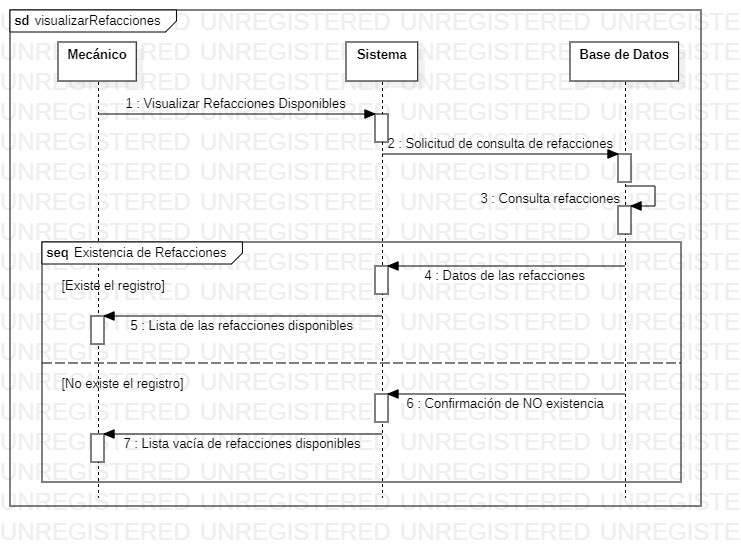
\includegraphics[width=1\textwidth]{./diseno/vprocesos/imagenes/visualizarRefacciones}
	\caption{Diagrama de Secuencia - Visualizar Refacciones}
	\label{fig:Diagrama de Secuencia - Visualizar Refacciones}
\end{figure}